\documentclass[12pt,oneside]{memoir} 

\usepackage[latinica, biblatex]{matfmaster} 
\usepackage{listings}
\usepackage{listings-golang}
\usepackage{color}
\usepackage{tikz}
\usepackage{pgfplots}
\usetikzlibrary{pgfplots.groupplots}
\usepackage{diagbox}
\usepackage{array}
\usepackage{fancyvrb}

\definecolor{background}{RGB}{255, 248, 220}


\lstset{ 
    frame=single,
    basicstyle=\footnotesize,
    keywordstyle=\color{blue},
    showstringspaces=false, 
    stringstyle=\color{red},
    tabsize=4,
    language=Golang
}

\lstnewenvironment{snippet}[1][]
    {\lstset{float=htpb,#1}} 
    {}



\bib{literatura}


\autor{Miloš Mitrović}
\naslov{Konkurentno programiranje u programskom jeziku Go}
\godina{2017}
\mentor{dr Milena \textsc{Vujošević Janičić}\\ Univerzitet u Beogradu, Matematički fakultet}
\komisijaA{dr Ana \textsc{Anić}\\  Univerzitet u Beogradu, Matematički fakultet}
\komisijaB{dr Laza \textsc{Lazić}\\  Univerzitet u Beogradu, Matematički fakultet}


\apstr{
text
}

\kljucnereci{programski jezik Go, konkurentno programiranje}

\begin{document}

\frontmatter
\naslovna
\komisija
\posveta{Mojoj sestri Ivoni}
\apstrakt
\tableofcontents*

\mainmatter

\chapter{Uvod}

% GO OPIS==============================================================================

\chapter{Karakteristike programskog jezika Go}

Go je imperativni programski jezik otvorenog koda koji razvija kompanija Google od 2007. godine. Napravljen je kao kompilirani jezik opšte namene sa statičkim tipovima koji podseća na interpretirane jezike sa dinamičkim tipovima. Podržava konkurentno programiranje, automatsko upravljanje memorijom kao i refleksiju tokom izvršavanja programa. Pogodan je za rešavanje svih vrsta problema a najviše se koristi za izgradnju servera, skriptove i samostalne aplikacije za komandnu liniju a može se korititi i za grafičke i mobilne aplikacije.

\section{Tipovi podataka}

Go je statički tipiziran jezik što znači da se varijabli dodeljuje tip prilikom njene deklaracije i on se ne može menjati tokom izvršavanja programa.  Za razliku od C-a Go ne podržava automatsku konverziju tipova već se konverzija mora navesti eksplicitno, u suprotnom se prijavljuje greška.\\

Od osnovnih ugrađenih tipova podataka Go podržava:
\begin{itemize}

\item Numeričke -  celobrojne označene (\texttt{int8}, \texttt{int16}, \texttt{int32}, \texttt{int64})
 i neoznačene  (\texttt{uint8}, \texttt{uint16}, \texttt{uint32}, \texttt{uint64}), u pokretnom zarezu (\texttt{float32}, \texttt{float64}) i kompleksne (\texttt{complex64}, \texttt{complex128})

\item Bulovske  (\texttt{bool})

\item Tekstualne (\texttt{string})

\end{itemize}

Od drugih vrsta podataka, Go podržava nizove, mape i slajseve - nizove sa promenljivom dužinom. Postoje i paketi koji omogućavaju rad sa listama.

\section{Funkcije i metodi}
 
\section{Interfejsi}

\section{Refleksija}

\section{Testiranje}

\section{Paketi}


% KONKURENTNO==============================================================================
\chapter{Konkurentno programiranje u programskom jeziku Go}

\section{Osnovni pojmovi konkurentnog programiranja}

\section{Mogućnosti u programskom jeziku Go}

\subsection{Go-rutine}

\subsection{Kanali}

\subsection{Sinhronizacija}

\subsection{Data race detektor}

\begin{figure}
\begin{center}

\begin{Verbatim}[fontsize=\small]
WARNING: DATA RACE
Write at 0x00c420072006 by goroutine 18:
  main.mark_prime()
      /home/cg/root/7238354/main.go:53 +0x1d8

Previous read at 0x00c420072006 by goroutine 83:
  [failed to restore the stack]

Goroutine 18 (running) created at:
  main.Prime()
      /home/cg/root/7238354/main.go:21 +0x1a0
  main.main()
      /home/cg/root/7238354/main.go:72 +0x126

Goroutine 83 (running) created at:
  main.Prime()
      /home/cg/root/7238354/main.go:21 +0x1a0
  main.main()
      /home/cg/root/7238354/main.go:72 +0x126
\end{Verbatim}

\caption{Primer upozorenja koje "data race" detektor daje za implementaciju Eratostenovog sita}
\label{fig:datarace}
\end{center}
\end{figure}

\subsection{Select naredba}


%PRIMERI ==============================================================================

\chapter {Primeri i poređenje sa drugim jezicima}
U ovom poglavlju su izloženi primeri konkurentnih Go programa i poređenje implementacija nekoliko jednostavnih algoritama u jezicima C, C++ i Python. Primeri ilustruju na koji način se može koristiti konkurentnost u jeziku Go i kakva je njegova efikasnost u odnosu na druge pomenute jezike. Prvo sledi kratak pregled programskih jezika C, C++ i Python i njihove konkurentnosti a zatim poređenje implementacija algoritama quicksort, množenje matrica i Eratostenovo sito.

\section{C}

\section{C++}

\section{Python}
\label{gil} GIL (Global Iinterpreter Lock) is a mutex that protects access to Python objects, preventing multiple threads from executing Python bytecodes at once.

\section{Osnovni primeri sa poređenjem}
Kao kriterijumi poređenja koriste se brzina izvršavanja, maksimalna upotreba memorije i broj linija k\^{o}da. Primeri su testirani na hardveru sa 48 jezgara pod Linux-om Ubuntu 16.04 ukoliko nije naglašeno suprotno. 



% Quicksort==============================================================================
\section{Quicksort}
Quicksort je algoritam za sortiranje brojeva u mestu koji spada u grupu algoritama podeli i vladaj. U svakom koraku, jedan element - pivot se postavlja na svoju poziciju u sortiranom nizu i deli se na dva podniza particionisanjem, jedan u kome su svi brojevi veći od pivota i drugi u kome su svi brojevi manji od pivota, koji se zatim sortiraju rekurzivno.  Pseudo kod algoritma je prikazan na slici \ref{fig:qs_pseudo}. 

Paralelizacija algoritma je izvršena tako što se za svaki rekurzivni poziv pokreće po jedna nit/rutina do određene granice kada se prelazi u sekvencijalni režim rada. Za testiranje su korišćeni pseudoslučajno generisani nizovi različitih dužina.

\begin{figure}
\begin{center}

\begin{Verbatim}[fontsize=\small]
algorithm quicksort(A, lo, hi):
    if lo < hi then
        p := partition(A, lo, hi)
        quicksort(A, lo, p - 1 )
        quicksort(A, p + 1, hi)

algorithm partition(A, lo, hi) :
    pivot := A[hi]
    i := lo - 1    
    for j := lo to hi - 1 do
        if A[j] < pivot then
            i := i + 1
            swap A[i] with A[j]
    if A[hi] < A[i + 1] then
        swap A[i + 1] with A[hi]
    return i + 1
\end{Verbatim}

\caption{Pseudokod algoritma quicksort}
\label{fig:qs_pseudo}
\end{center}
\end{figure}


\subsection{Go}
\label{qs:go}
Implementacija \ref{lst:qs} koristi koncept višestrukog semafora za ograničavanje broja aktivnih go-rutina. Semafor je realizovan pomoću kanala sa baferom i select naredbe gde kapacitet kanala označava maksimalan broj aktivnih go-rutina. U select naredbi se pokušava "dobijanje tokena" odnosno slanje poruke kroz kanal sa baferom. Kanal je definisan nad tipom prazne strukture jer nam nije bitna sama poruka već samo trenutno zauzeće kanala. U slučaju da možemo da dobijemo token odnosno uspešno pošaljemo praznu strukturu kroz kanal pokrećemo go-rutinu za rekurzivni poziv, u suprotnom, ukoliko nema slodbnog mesta u baferu, rekurzivni poziv se izvršava sekvencijalno. Na kraju svake go-rutine je potrebno pročitati poruku iz kanala odnosno osloboditi jedno mesto. Da bismo bili sigurni da su sve go-rutine završile sa svojim radom, za sinhronizaciju koristimo wait grupe. Svaki konkurentni poziv funkcije kreira svoju wait grupu kojoj postavlja brojač na dva, a zatim, na kraju, čeka da oba rekurzivna poziva završe sa radom. S obzirom da unapred nije poznato kada će moći da se izvrši konkurentni a kada sekvencijalni poziv funkcije, potrebno je u oba slučaja signalizirati wait grupi da je završeno sa radom. Niz se prenosi preko reference i nije potrebno nikakvo zaključavanje jer svaki poziv fununkcije menja samo svoj deo niza.

\begin{center}
\begin{lstlisting}[caption=Go implementacija konkurentne quicksort funkcije,label={lst:qs},float,  backgroundcolor=\color{background}]
var semaphore = make(chan struct{}, 100)

func QuickSortConcurrent(a *[]int, low, hi int) {
	if hi < low {
		return
	}

	p := partition(a, low, hi)

	wg := sync.WaitGroup{}
	wg.Add(2)

	select{
	case semaphore <- struct{}{}:
		go func(){
			QuickSortConcurrent(a, low, p-1)
			<- semaphore
			wg.Done()
		}()
	default:
		QuickSortSequential(a,low, p-1)
		wg.Done()
	}

	select{
	case semaphore <- struct{}{}:
		go func(){
			QuickSortConcurrent(a, p+1, hi)
			<- semaphore
			wg.Done()
		}()
	default:
		QuickSortSequential(a, p+1, hi)
		wg.Done()
	}

	wg.Wait()
}
\end{lstlisting}
\end{center}

\subsection{C}
Za razliku od Go implementacije, ovde je upotrebljena dubina rekurzije za ograničavanje broja niti koje program kreira. Kada se dostigne zadata dubina rekurzije program više ne kreira nove niti već prelazi u sekvencijalni režim rada. Svaki konkurentni poziv funkcije kreira po dve nove niti ukoliko maksimalna dubina nije dostignuta, nakon čega se join funkcijom čeka na njihov završetak sa radom.

\subsection{C++}
Za C++ su razmatrane dve implementacije: prva, u kojoj je niz reprezentovan strukturom vektor i koristi standardnu biblioteku, i druga, koja koristi običan niz int-ova i OpenMP biblioteku. 
Prva implementacija ima koncept dubine rekurzije za restrikciju broja niti na isti način kao što je realizovano u C-u. Druga, u kojoj je upotrebljena OpenMP biblioteka, ima mogućnost da postavi maksimalni broj aktivnih niti u jednom trenutku.

\subsection{Python}
Ovde se takođe razmatraju dve implementacije koje koriste različite pakete za realizaciju konkurentnosti. Kod prve implementacije koristi se threading paket i postavlja se maksimalni broj aktivnih niti. U drugoj verziji je iskorišćen Parallel Python paket sa već pomenutim konceptom dubine rekurzije za kontrolu broja niti. 

\subsection{Rezultati}\label{qs:rez}

Vremenska efikasnost implementacija u zavisnosti od veličine niza je prikazana u tabeli \ref{tab:qs1}.  C i C++ OpenMP implementacija su se pokazale kao najefikasnije. Vreme izvršavanja Go implementacije je uporedivo za nizove od milion i 10 miliona dok je za niz od 100 miliona brojeva potrebno dva puta više vremena u odnosu na C i C++ OpenMP implementacije. C++ verzija sa standardnom bibliotekom je značajno sporija od pomenutih implementacija, ali je Python-u potrebno najviše vremena i nije bilo mogućnosti testirati ga za niz od 100 miliona brojeva.

U odnosu na sekvencijalno izvršavanje, najveće ubrzanje ima C. Sekvencijalno se najbrže izvršava Go i za niz od milion brojeva mu je potrebno isto vremena kao i pri konkurentnom izvršavanju.  Ubrzanje se vidi za nizove veće dužine međutim ono je manje u odnosu na C i C++ OpenMP verziju. C++ implementacija sa standardnom bibliotekom nema nikakvo ubrzanje kada je testirano na već pomenutom hardveru sa 48 jezgara. Međutim, testirano na drugom računaru pokazalo se da postoji ubrzanje od približno 50\% kada se izvršava konkurentno. Napomena da rezultati dobijeni testiranjem na drugom računaru služe samo kao relativan odnos sekvencijalnog i konkurentog izvršavanja, a ne za poređenje sa drugim implementacijama, usled različite brzine izvršavanja.

Kod Python threading implementacije, konkurentno izvršavanje je sporije u odnosu na sekvencijalno kao direktna posledica GIL-a što je objašnjeno u odeljku \ref{gil}. Verzija koja koristi Parallel Python paket pokazuje da je moguće napraviti konkurentan program sa nitima u Pythonu koji je efikasniji u odnosu na sekvencijalno izvršavanje. Međutim i ova verzija je višestruko sporija u odnosu na implementacije u drugim jezicima. 

\begin{table}
\begin{center}
\caption{Vreme izvršavanja [s] quicksort implementacija za različito n, testirano sa 48 jezgara}
\begin{tabular}{||c||c|c|c||c|c|c||}
\hline
&\multicolumn{3}{c||}{Konkurentno izvršavanje}&\multicolumn{3}{c||}{Sekvencijalno izvršavanje} \\ \hline
\diagbox[width=2.7cm, height=1cm]{Verzija}{\vspace*{-0.8cm}n [$10^{6}$]} &1 &10 &100 &1 &10 &100 \\ \hline
C 		&\textbf{ 0.33}	&2.68			&\textbf{14.29}	& 0.63 		&  2.90		&58.86		\\ 
C++ omp	& 0.87		&\textbf{2.58}	&15.22		& 0.68		&\textbf{2.64} 	&50.66  		\\ 	
Go		& 0.49  		&2.71			&29.36		& \textbf{0.48}	&  4.22 		& \textbf{43.70}	\\ 
C++ std	& 1.37		&15.50		&172.23		& 1.47 		& 15.53		&173.68		\\ 
Python thr	& 28.98		&340.82		& - 			& 9.71		& 135.32		& - 			\\ \hline
C++ std\textsuperscript{*}	& 0.35		&3.52			& 60.96		& 0.68 		& 7.80		&98.74		\\
Python pp\textsuperscript{*}	& 4.35		&58.87		& - 			& 8.46		& 118.33		& - 			\\ \hline
\multicolumn{7}{l}{\textsuperscript{*}\footnotesize{Testirano na dva jezgra/četiri niti pod Linux-om Ubuntu 17.04}}
\end{tabular}
\label{tab:qs1}
\end{center}
\end{table}

Vremenska efikasnost implementacija u zavisnosti od broja jezgara koji se koristi za izvršavanje, za niz od 10 miliona brojeva je prikazana na slici \ref{fig:qs1}. Python nije testiran jer broj jezgara ne utiče na njegovu brzinu izvršavanja. C++ verzija sa OpenMP bibliotekom jedina ima strogo opadajuću krivu, odnosno sa većim brojem jezgara potrebno joj je manje vremena. Go i C ne osciluju značajno, osim što rade nešto sporije sa 16 i 24 jezgara, nema velike razlike u brzini sa 4 i 48 jezgara. Broj jezgara ne utiče na C++ verziju sa standardnom bibliotekom jer kao što je i prethodno testiranje pokazalo na ovom računaru konkurentno izvršavanje ne donosi nikakvo ubrzanje. 

\begin{figure}
\begin{center}

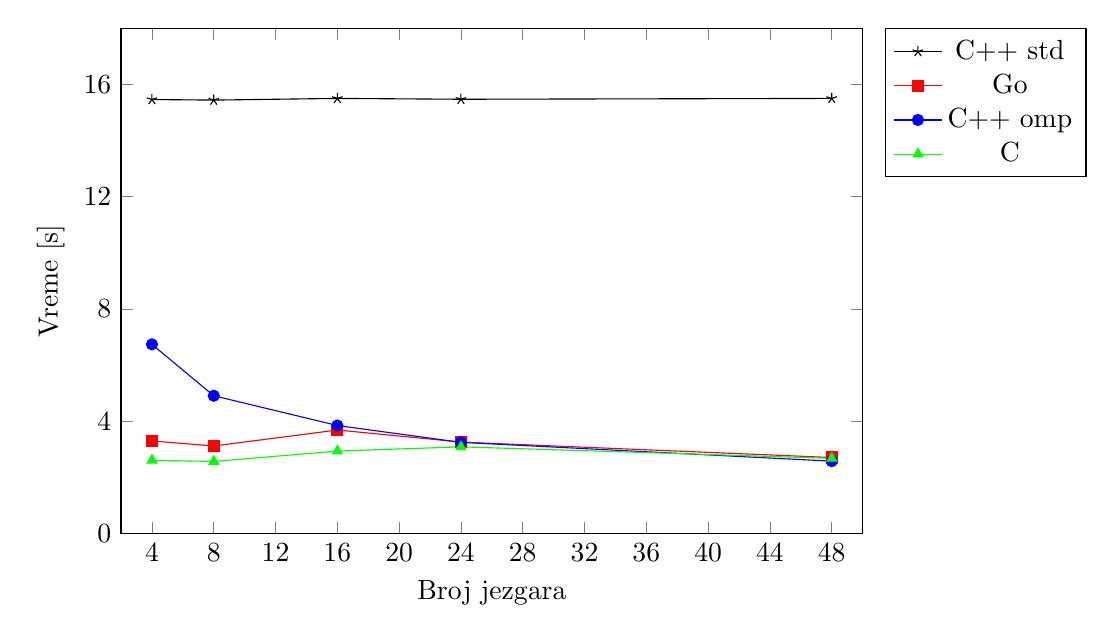
\begin{tikzpicture}
\begin{axis}[
    xlabel={Broj jezgara},
    ylabel={Vreme [s]},
    xmin=2, xmax=50,
    ymin=0, ymax=18,
    xtick={4,8,12,16,20,24,28,32,36,40,44,48},
    ytick={0,4,8,12,16},
    legend pos=outer north east,
    ymajorgrids=true,
    grid=none,
    width=11cm,
    height=8cm,
]

\addplot[black,mark=star] coordinates {(4,15.46)(8,15.44)(16,15.50 )(24,15.47 )(48,15.50)};  
\addplot[red,mark=square* ]  coordinates {(4,3.30)(8,3.12)(16,3.69 )(24,3.26)(48,2.71)}; 
\addplot[blue,mark=*]  coordinates {(4,6.74)(8,4.91)(16,3.85 )(24,3.25 )(48,2.58)}; 
\addplot[green,mark=triangle*] coordinates {(4,2.61)(8,2.57)(16,2.94 )(24,3.09 )(48,2.68)};

\legend{ C++ std, Go,C++ omp,C}
\end{axis}
\end{tikzpicture}

\caption{Grafik brzine izvršavanja različitih quicksort implementacija u zavisnosti od broja jezgara, testirano za niz od 10 miliona brojeva}
\label{fig:qs1}
\end{center}
\end{figure}

Maksimalna upotreba memorije za nizove različitih dužina je prikazana u tabeli \ref{tab:qs3}. Obe verzije u C++-u su podjednako efikasne i potrebno im je najmanje memorije u odnosu na druge implementacije. C je približno efikasan kao i C++ osim što i za nizove manjih dužina zahteva veliku količinu memorije. Go koristi dva puta više memorije nego ostale implementacije dok je Pythonu potrebna višestruko veća količina memorije.

\begin{table}
\begin{center}
\caption{Maksimalna upotreba memorije [MB] quicksort implementacija za različite dužine niza}
\begin{tabular}{||c||c|c|c||}
\hline
\diagbox[width=2.7cm, height=1cm]{Verzija}{\vspace*{-0.8cm}n [$10^{6}$]} &1 &10 &100 0 \\ \hline
C++ omp	& \textbf{6.3}	&42.3			&\textbf{393.1}	\\ 	
C++ std	& 6.7			&\textbf{42.0}	&393.5		\\ 
C 		& 58.1		&68.8			&408.5		\\ 
Go		& 13.4 		&87.5			&816.3		\\ 
Python thr	& 40.4		&396.3		& -			\\
Python pp	& 49.6		&411.8		& - 			\\ \hline
\end{tabular}
\label{tab:qs3}
\end{center}
\end{table}

Dužine programskih kodova se mogu pogledati u tabeli \ref{tab:qs4}. U C-u je potrebno najviše linija  k\^{o}da za implementaciju algoritma dok je u Pythonu potrebno najmanje.

\begin{table}
\begin{center}
\caption{Dužine k\^{o}da quicksort implementacija}
\begin{tabular}{|c|c|c|c|c|c|c|}
\hline
		&  C 	& Go	& C++ std	& C++ omp	& Python pp & Python thr \\ \hline
Br. linija koda& 119	& 98	&84		&79		&55		&43	 \\ \hline
\end{tabular}
\label{tab:qs4}
\end{center}
\end{table}

\subsection{Zaključak}

Na ovom primeru Go se pokazao vremenski efikasan isto koliko i C i C++ za nizove dužine do 10 miliona dok mu je potrebno dva puta više vremena za nizove dužine od 100 miliona, ali se prilkom sekvencijalnog izvršavanja ispostavio kao najefikasniji. Potrebno mu je dva puta više memorije nego C-u i C++-u ali je i memorijski i vremenski višestruko efikasniji od Pythona.  Dužina koda je uporediva sa C-om i C++-om.

% Matrix==============================================================================

\section{Množenje matrica}
Implementiran je standardni algoritam za množenje matrica. Vrednost na poziciji \textit{ij} proizvoda matrica A i B se izračunava kao: $$(AB)_{ij} = \sum_{k=1}^{n} A_{ik}B_{kj}$$ gde je n dužina matrice A. 

Algoritam je paralelizovan tako što svaka nit/rutina računa po jedan red matrice, odnosno jedan red prve matrice množi sa svim kolonama druge matrice. Za testiranje su korišćene pseudoslučajno generisane kvadratne matrice različitih dimenzija. 

\subsection{Go}
Restrikcija broja go-rutina se ostvaruje pomoću semafora na isti način kao što je urađeno u prethodnom primeru \ref{qs:go}. Može se primetiti u implementaciji \ref{lst:matrix} da je neophodno go-rutinama  proselditi \textit{i} kao argument anonimne funkcije kako bi svaka imala svoju kopiju. U suprotnom, u svakoj sledećoj iterciji for petlje vrednost \textit{i} bi bila ažurirana u svim go-rutinama. Za razliku od prethodnog primera gde se niz koji se sortira prenosi pomoću reference, ovde su rezultujuća i početne matrice definisane kao globalne. Ni u ovom slučaju nije potrebno zaključavanje jer se početne matrice koriste samo za čitanje, a kod rezultujuće matrice svaka go-rutina popunjava samo svoj red. 

\begin{center}
\begin{lstlisting}[caption=Go implementacija konkurentne funkcije za množenje matrica,label={lst:matrix},float, backgroundcolor=\color{background}]
func multiply(){
	wg := sync.WaitGroup{}
	wg.Add(n)

	for i := 0; i < n; i++ {
		select{
		case semaphore <- struct{}{}:
			go func(row int){
				multiply_row(row)
				<- semaphore
				wg.Done()
			}(i)
		default:
			multiply_row(i)
			wg.Done()
		}
	}

	wg.Wait()
}
\end{lstlisting}
\end{center}

\subsection{Ostale implementacije}
Implementacije u ostalim jezicima su realizovane na sličan način. Maksimalan broj niti koji se kreira u toku izvršavanja programa se unapred zadaje. Za C++ razmatrane su dve implementacije. Jedna je ostvarena pomoću OpenMP biblioteke i koristi običan niz za reprezntaciju matrice, dok druga koristi strukturu vektor i standardnu biblioteku.


\subsection{Rezultati}

Grafik brzine izvršavanja u zavisnosti od veličine matrice je prikazan na slici \ref{fig:matrix1}. Python se izvršava znatno sporije od ostalih implementacija tako da nije bilo mogućnosti testirati ga na ulazima iste veličine, a rezultati testiranja Python implementacije su prikazani u tabeli \ref{tab:matrix1}. Na grafiku se vidi da je C implementacija najefikasnija, a zatim C++ verzija sa OpenMP bibliotekom, dok verzija sa standardnom bibliotekom radi najsporije. Za matrice manje veličine Go radi podjednako efikasno kao i OpenMP verzija C++ implementacije, ali za matricu veličine 1500 mu je potrebno dva puta više vremena, što je približno četiri puta više nego C-u. 

\begin{figure}
\begin{center}

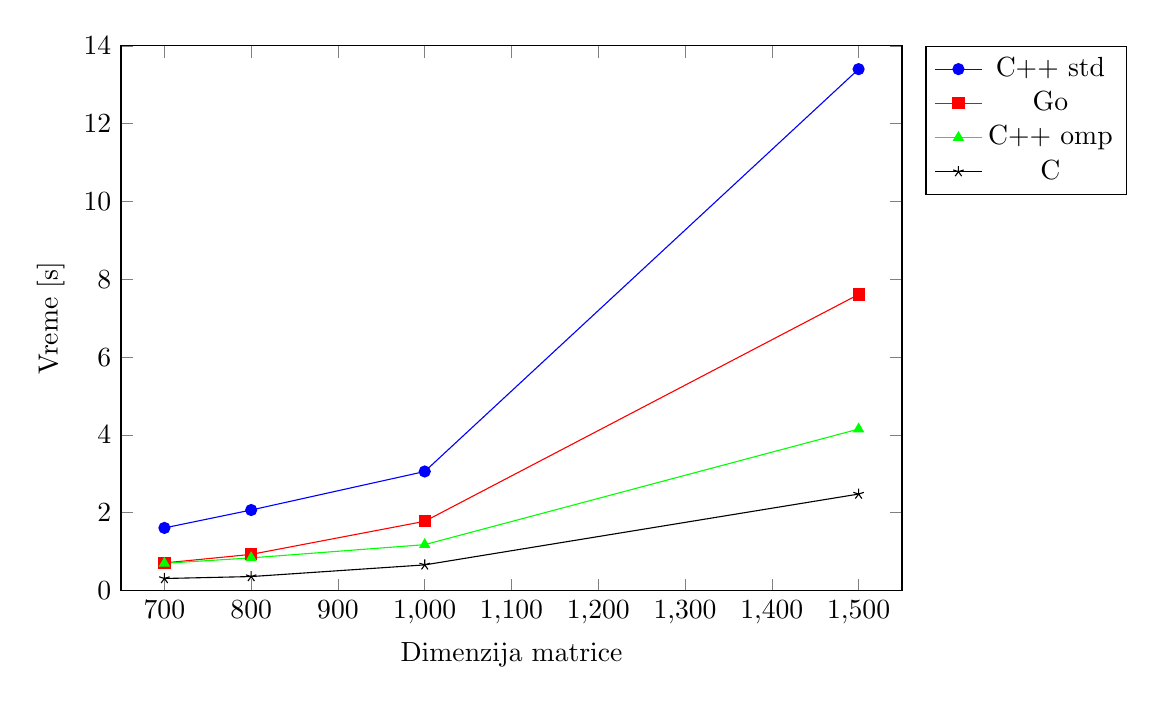
\begin{tikzpicture}
\begin{axis}[
    xlabel={Dimenzija matrice},
    ylabel={Vreme [s]},
    xmin=650, xmax=1550,
    ymin=0, ymax=14,
    xtick={700,800,900,1000,1100,1200,1300,1400,1500},
    ytick={0,2,4,6,8,10,12,14,16,18,20,22},
    legend pos=outer north east,
    ymajorgrids=true,
    grid=none,
    width=11.5cm,
    height=8.5cm,
]

\addplot[blue,mark=*] coordinates {(700,1.61 )(800,2.07 )(1000,3.06 )(1500,13.4 )}; 
\addplot[red,,mark=square*] coordinates {(700,0.71 )(800,0.93 )(1000,1.78 )(1500,7.61 )}; 
\addplot[green,mark=triangle*] coordinates {(700,0.70 )(800,0.84 )(1000,1.18 )(1500,4.15 )}; 
\addplot[black,mark=star] coordinates {(700, 0.31)(800, 0.36)(1000, 0.66)(1500,2.48 )}; 
\legend{C++ std,Go, C++ omp,C}
\end{axis}
\end{tikzpicture}

\caption{Grafik brzine izvršavanja različitih implementacija množenja matrica u zavisnosti od veličine matrice, testirano na 48 jezgara}
\label{fig:matrix1}
\end{center}
\end{figure}

Rezultati testiranja implementacija na različitom broju jezgara prikazani su na slici \ref{fig:matrix3}. Na grafiku se vidi velika razlika u brzini između sekvencijalnog (na jednom jezgru) i konkurentnog izvršavanja. Brzina raste do 16 i 24 jezgara, dok povećanje na 48 jezgara, ne donosi značajno ubrzanje. 

\begin{figure}
\begin{center}

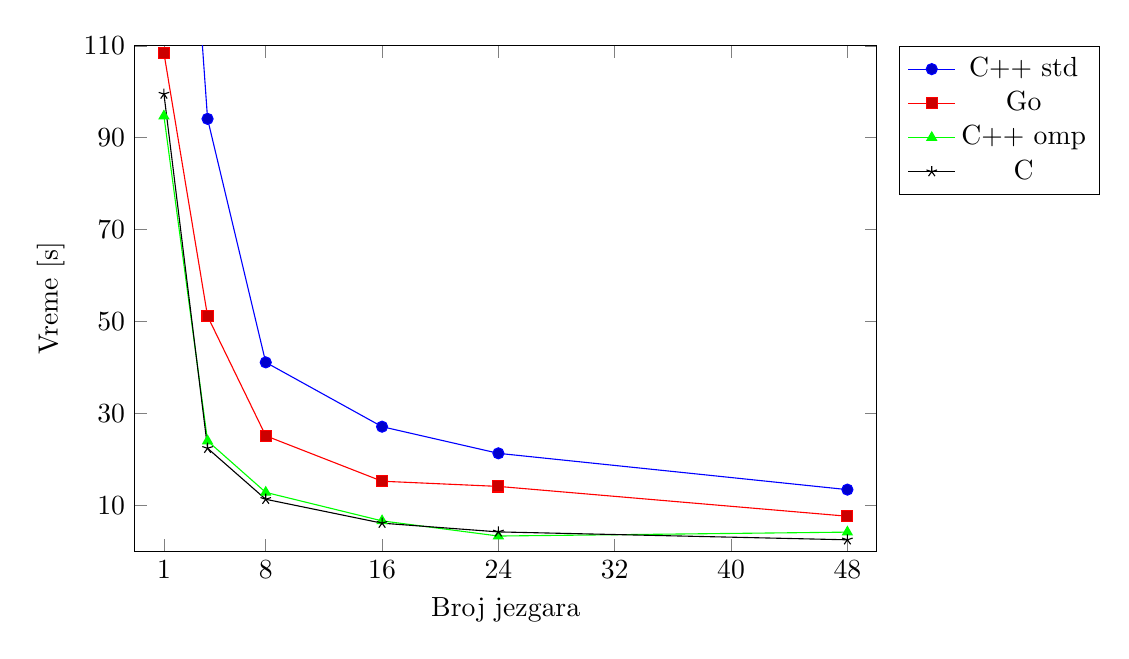
\begin{tikzpicture}
\begin{axis}[
    xlabel={Broj jezgara},
    ylabel={Vreme [s]},
    xmin=-1, xmax=50,
    ymin=0, ymax=110,
    xtick={1,8,16,24,32,40,48},
    ytick={10,30,50,70,90,110},
    legend pos=outer north east,
    ymajorgrids=true,
    grid=none,
    width=11cm,
    height=8cm,
]
\addplot coordinates {(1, 229)(4,94.1)(8,41.1)(16,27.1 )(24,21.3 )(48,13.4)}; 
\addplot coordinates {(1,108.4 )(4,51.14)(8,25.12)(16,15.23 )(24,14.1 )(48,7.61)}; 
\addplot[green,mark=triangle*]  coordinates {(1,94.7 )(4,24)(8,12.8)(16,6.6 )(24,3.3 )(48,4.15)}; 
\addplot coordinates {(1,99.5 )(4,22.4)(8,11.3)(16,6.1 )(24,4.2 )(48,2.48)}; 


\legend{C++ std, Go, C++ omp, C}
\end{axis}
\end{tikzpicture}

\caption{Grafik brzine izvršavanja različitih implementacija množenja matrica u zavisnosti od broja jezgara za matricu veličine 1500}
\label{fig:matrix3}
\end{center}
\end{figure}

Python se izvršava višestruko sporije i potrebno mu je više od 90 sekundi za matricu veličine 500, dok je ostalim implementacijama potrebno manje od jedne sekunde. Konkurentno izvršavanje je ponovo sporije od sekvencijalnog zbog već pomenutog problema sa GIL-om u odeljku \ref{gil}. Rezultati su prikazani u tabeli \ref{tab:matrix1}.

\begin{table}
\begin{center}
\caption{Vreme izvršavanja i maksimalna upotreba memorije Python implementacije množenja matrica za različito n}
\begin{tabular}{||c||c|c|c||}
\hline
n & Konkurentno [s]& Sekvencijalno [s] & Memorija [MB] \\ \hline
100	&0.78	&0.32&7.5\\
300	&21.11&7.59&10.0\\
500	&97.73&38.27&17.4\\
\hline
\end{tabular}
\label{tab:matrix1}
\end{center}
\end{table}


Grafik maksimalne upotrebe memorije u zavisnosti od dimenzije matrica je prikazan na slici \ref{fig:matrix2}. Memorijska efikasnost se u ovom primeru poklapa sa vremenskom. C i C++ OpenMP vezija su najefikasnije dok Go koristi dva puta više memorije. C++ verzija sa standardnom bibliotekom zahteva najveću količinu memorije. 

\begin{figure}
\begin{center}

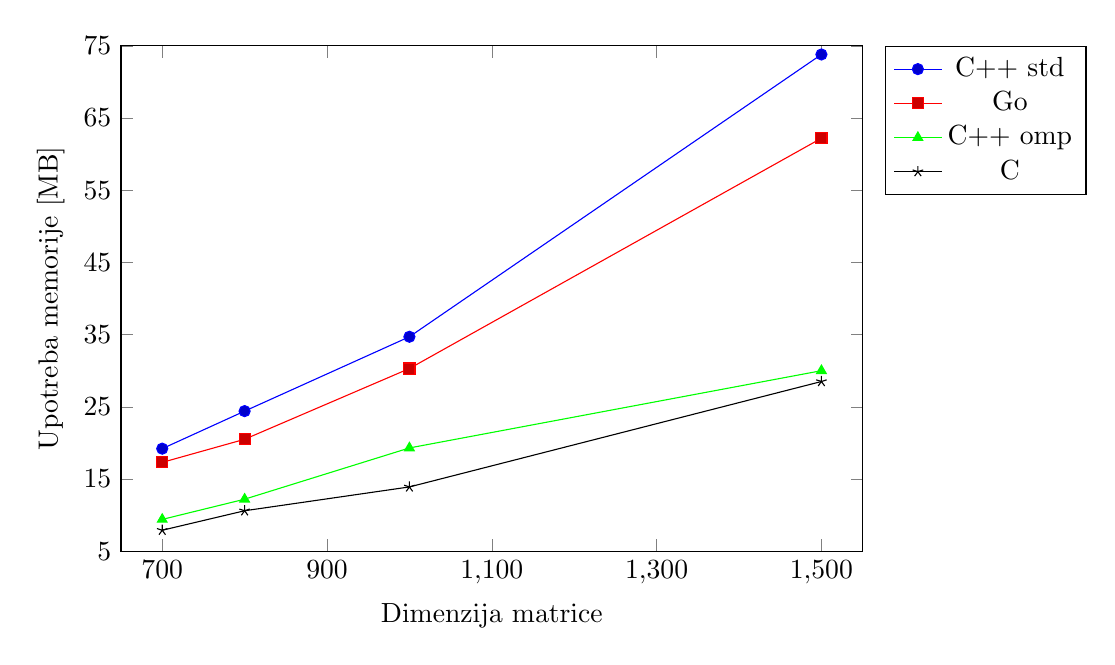
\begin{tikzpicture}
\begin{axis}[
    xlabel={Dimenzija matrice},
    ylabel={Upotreba memorije [MB]},
    xmin=650, xmax=1550,
    ymin=5, ymax=75,
    xtick={700,900,1100,1300,1500},
    ytick={5,15,25,35,45,55,65,75},
    legend pos=outer north east,
    ymajorgrids=true,
    grid=none,
    width=11cm,
    height=8cm,
]
\addplot coordinates {(700, 19.2)(800, 24.4)(1000, 34.7)(1500,73.8 )}; 
\addplot coordinates {(700,17.3 )(800,20.5 )(1000,30.3 )(1500,62.2)}; 
\addplot[green,mark=triangle*] coordinates {(700,9.4 )(800,12.2 )(1000,19.3 )(1500,30 )}; 
\addplot[black,mark=star] coordinates {(700,7.9 )(800,10.6 )(1000,13.9)(1500,28.5)}; 
\legend{ C++ std,Go, C++ omp,C}
\end{axis}
\end{tikzpicture}

\caption{Grafik maksimalne upotrebe memorije različitih implementacija množenja matrica u zavisnosti od dimenzije matrica}
\label{fig:matrix2}
\end{center}
\end{figure}


Broj linija k\^{o}da svih  implementacija je prikazan u tabeli \ref{tab:matrix2}. Python ima najkraću implementaciju sa samo 28 linija k\^{o}da. Najduža implementacija je C++ verzija sa standardnom bibliotekom jer je razdvojena na klase i nekoliko fajlova radi jednostavnijeg korišćenja.  

\begin{table}
\begin{center}
\caption{Dužine k\^{o}da implementacija množenja matrica}
\begin{tabular}{|c|c|c|c|c|c|}
\hline
		& C++ std	&  Go 	& C	& C++ omp	& Python	\\ \hline
Br. linija koda&170		& 75	& 70	&50		&28		\\ \hline
\end{tabular}
\label{tab:matrix2}
\end{center}
\end{table}

\subsection{Zaključak}

Go se ponovo pokazao vremenski efikasan koliko C i C++ za ulaze manjih dimenzija, dok za velike ulaze zahteva dva puta više vremena. Takođe, potrebna mu je dva puta veća količina memorije ali je neuporedivo vremenski i memorijski efikasniji od Python-a. Potreban je približno isti broj linija k\^{o}da za implementaciju algoritma koliko i u C-u.


% Prime==============================================================================

\section{Eratostenovo sito}
Eratostenovo sito je algoritam za određivanje prostih brojeva manjih od n. Ideja algoritma je da se elimnišu svi brojevi koji nisu prosti između 2 i n. Na početku se pretpostavlja da su svi brojevi prosti odnosno definiše se niz od n bulovskih vrednosti postavljenih na true. Kreće se od prvog prostog broja što je 2 tako što se eliminiše svaki drugi broj počevši od $2^{2}$, a zatim se prelazi na sledeći prost broj i postupak se ponavlja. Uopšteno, za i-ti prost broj eliminiše se svaki i-ti broj počevši od  $i^{2}$. Postupak je dovoljno ponoviti za proste brojeve koji su manji od $\sqrt{n}$. Pseudokod algoritma je prikazan na slici \ref{fig:prime_pseudo}.

\begin{figure}
\begin{center}

\begin{Verbatim}[fontsize=\small]
for i:=2 to n do
    A[i]:=true

ErathostenesSieve(n):
    for i:=2 to floor(sqrt(n)) do 
         if A[i] = true:
             j := i * i
             while j < n do
                 A[j] := false 
                 j := j + i
\end{Verbatim}

\caption{Pseudokod algoritma Eratostenovo sito}
\label{fig:prime_pseudo}
\end{center}
\end{figure}

Paralelizacija algoritma se postiže deljenjem opsega od 2 do n na jednake delove. Svaka nit/rutina dobija svoj deo opsega u okviru kojeg eliminiše brojeve koji nisu prosti. Za svaki prost broj je prvo potrebno odrediti njegov prvi umnožak unutar opsega. Iako svaka nit/rutina ima svoj opseg, ona mora da pristupa članovima niza drugih niti/rutina jer su joj potrebni svi prosti brojevi manji od $\sqrt{n}$. To kao posledicu dovodi do mogućnosti da se u nekim slučajevima bespotrebno eliminišu umnošci brojeva koji nisu prosti ukoliko ih druga nit/rutina još uvek nije eliminisala. Problem je rešen tako što se proverava dodatni uslov prilikom eliminacije: da li je neka druga nit/rutina u međuvremenu označila da taj broj nije prost.


\subsection{Go}

Koristi se globalni niz od n bulovskih promenljivih postavljenih na podrzumevanu vrednost - false umesto na true radi jednostavnosti.  Funkcija koja kreira go-rutine je prikazana u listingu \ref{lst:prime1}. Za svaki broj koji je trenutno označen kao prost, najpre je potrebno je odrediti njegov prvi umnožak, a zatim, označiti sve njegove umnoške unutar opsega, što je i prikazano u listingu \ref{lst:prime2}. Kao što je već pomenuto, ako svaka go-rutina ima svoj opseg, ona mora da pristupa i članovima niza drugih go-rutina jer su joj potrebni svi prosti brojevi manji od $\sqrt{n}$. To kao posledecu dovodi do pojave data race-a, međutim, u ovom slučaju je to dopustivo i nisu potrebni muteksi upravo zato što proveravamo dodatni uslov da li je pročitana vrednost u međuvremenu bila menjana. Ako se data race detektor pozove, dobija se izveštaj koji upozorava da postoji data race. Primer izveštaja se može videti na slici \ref{fig:datarace}. 

\begin{center}
\begin{lstlisting}[caption=Go implementacija konkurentne funkcije za određivanje prostih brojeva manjih od n,label={lst:prime1},float, backgroundcolor=\color{background}]
func Prime(list *[]bool, n int, is_concurrent bool){
	sqrt := int(math.Sqrt(float64(n)))
	first := 0
	step := int(n/ num_goroutines)
	last := step
	wg := sync.WaitGroup{}
	wg.Add(num_goroutines)

	for i:=0; i < num_goroutines-1; i++{
		go mark_prime(list,first,last,sqrt,&wg,true)
		first = last + 1
		last += step
	}

	mark_prime(list,first,n-1,sqrt,&wg)
	wg.Wait()
}
\end{lstlisting}
\end{center}

\begin{center}
\begin{lstlisting}[caption=Go implementacija konkurentne funkcije za označavanje prostih brojeva,label={lst:prime2},float, backgroundcolor=\color{background}]
func mark_prime(list *[]bool,first,last,sqrt int,wg *sync.WaitGroup){
	for i:=2;  i<= sqrt && i*i<= last; i++{
		if !(*list)[i] {
			var j int
			if i*i < first {
				if (first - i*i)%i == 0 {
					j = i*i + ((first-i*i)/i)*i
				}else {
					j = i*i + ((first-i*i)/i + 1)*i
				}
			}else {
				j = i*i
			}
		
			for ; j <= last && !(*list)[i]; j+=i {
				(*list)[j] = true
			}
		}
	}
	wg.Done()
}
\end{lstlisting}
\end{center}

\subsection{Ostale implementacije}
Implementacije u ostalim jezicima su realizovane na isti načini. Za C++ je razmatrana samo jedna implementacija koja koristi OpenMP biblioteku.

\subsection{Rezultati}

Vreme konkurentnog i sekvencijalnog izvršavanja implementacija je predstavljeno grafikom na slici \ref{fig:prime1}. Python ponovo nije mogao da bude uključen usled znatno sporijeg izvršavanja, a rezultati su prikazani u tabeli \ref{tab:prime1}. Go implementacija se pokazala kao najefikasnija a zatim implementacija u C++-u. C je znatno sporiji i njegovo izvršavanje se meri u sekundama dok Go i C rade ispod jedne sekunde. U odnosu na sekvencijano izvršavanje, Go ima najveće ubrzanje. Pri konkurentnom izvršavanju, veličina ulaza nema značajan uticaj tako da za Go i C++ nema velike razlike u brzini kada n iznosi 500 miliona ili 1 bilion. 


\pgfplotsset{ every non boxed x axis/.style={} }

\begin{figure}
\begin{center}

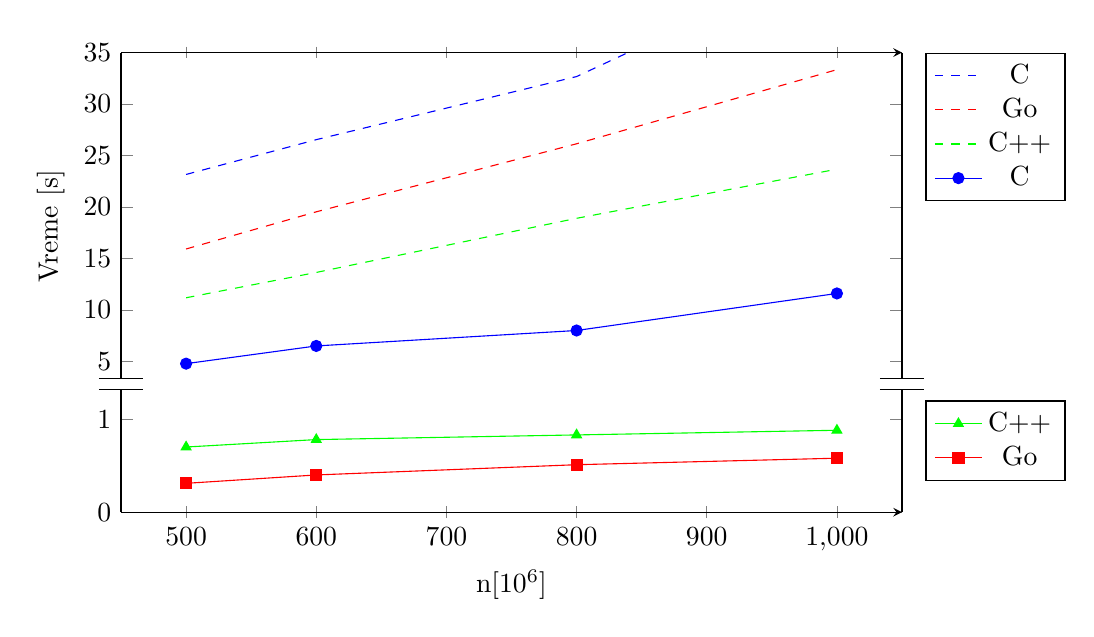
\begin{tikzpicture}
\begin{groupplot}[
    group style={
        group name=my fancy plots,
        group size=1 by 2,
        xticklabels at=edge bottom,
        vertical sep=0cm
    },
    xlabel={n[$10^{6}$]},
    ylabel={Vreme [s]},
    xmin=450, xmax=1050,
    xtick={500,600,700,800,900,1000},
    legend pos=outer north east,
    ymajorgrids=true,
    grid=none,
    width=11.5cm,
]


\nextgroupplot[ymin=1.2,ymax=35,
               ytick={5,10,15,20,25,30,35},
               axis x line=top, 
               axis y discontinuity=parallel,
               height=6.0cm,
	    xlabel={}]

\addplot[blue, dashed] coordinates {(500,23.16 )(600,26.54)(800,32.67 )(1000, 44.47)};
\addplot[red, dashed] coordinates {(500, 15.92 )(600,19.53)(800,26.14 )(1000, 33.34)};   
\addplot[green, dashed] coordinates {(500, 11.18 )(600,13.64)(800,18.9 )(1000, 23.67)};
\addplot[blue,mark=*] coordinates {(500,4.78 )(600,6.5)(800,8 )(1000, 11.6)}; 
\legend{C,Go,C++,C}


\nextgroupplot[ymin=0,ymax=1.2,
               ytick={0,1},
               axis x line=bottom,
               height=3.0cm, ylabel={}]


\addplot[green,mark=triangle*] coordinates {(500, 0.7)(600,0.78)(800,0.83 )(1000,0.88 )}; 
\addplot[red,mark=square*] coordinates {(500,0.31 )(600,0.4)(800,0.51 )(1000,0.58 )}; 
\legend{C++,Go}

\end{groupplot}
\end{tikzpicture}

\caption{Grafik brzine izvršavanja različitih implementacija Eratostenovog sita za različito n, testirano na 48 jezgara; isprekidanom linjom je prikazano sekvencijalno izvršavanje dok je konkurentno prikazano punom linijom}
\label{fig:prime1}

\end{center}
\end{figure}

Grafik brzine izvršavanja implementacija u zavisnosti od broja jezgara je prikazan na slici \ref{fig:prime3}. Za Go i C++ je potrebno manje vremena za izvršavanje sa većim brojem jezgara, međutim povećanje sa 24 na 48 jezgara ne donosi značajno ubrzanje. Pokazalo se da C radi sporije sa 8 i 16 jezgara nego sa 4, ali je ipak najefikasniji sa 48 jezgara. 


\begin{figure}
\begin{center}

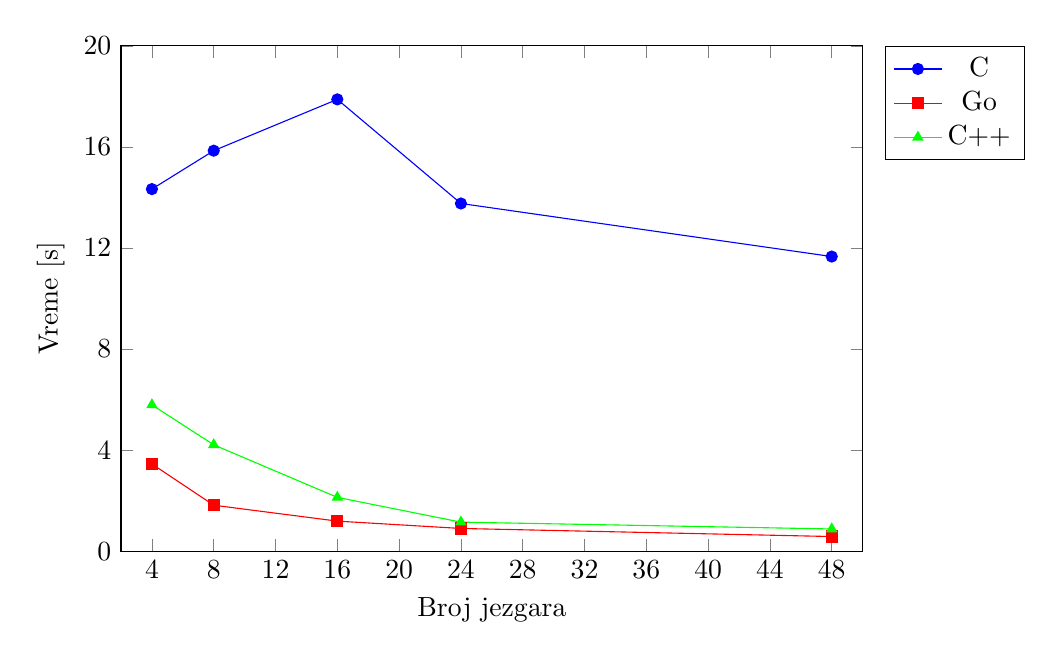
\begin{tikzpicture}
\begin{axis}[
    xlabel={Broj jezgara},
    ylabel={Vreme [s]},
    xmin=2, xmax=50,
    ymin=0, ymax=20,
    xtick={4,8,12,16,20,24,28,32,36,40,44,48},
    ytick={0,4,8,12,16,20},
    legend pos=outer north east,
    ymajorgrids=true,
    grid=none,
    width=11cm,
    height=8cm,
]
\addplot[blue,mark=*] coordinates {(4,14.33)(8,15.85)(16,17.88 )(24,13.76 )(48,11.66)}; 
\addplot[red,mark=square* ]   coordinates {(4,3.45)(8,1.82)(16,1.19 )(24,0.90 )(48,0.58)}; 
\addplot[green,mark=triangle*] coordinates {(4,5.79)(8,4.21)(16,2.13 )(24,1.15)(48,0.88)}; 
\legend{C, Go, C++}
\end{axis}
\end{tikzpicture}

\caption{Grafik brzine izvršavanja različitih implementacija Eratostenovog sita u zavisnosti od broja jezgara}
\label{fig:prime3}
\end{center}
\end{figure}

Python je testiran za 10 puta manju vrednost n u odnosu na ostale implementacije i potrebno mu je više od jednog minuta, dok Go za 10 puta veću vrednost radi ispod jedne sekunde. Upotreba memorije je 4 puta veća nego kod ostalih implementacija i potrebno mu je više vremena pri konkurentnom izvršavanju nego pri sekvencijalnom usled već pomenutog problema sa GIL-om u odeljku \ref{gil}.

\begin{table}
\begin{center}
\caption{Vreme izvršavanja i maksimalna upotreba memorije Python implementacije Eratostenovog sita za različito n}
\begin{tabular}{||c||c|c|c||}
\hline
n[$10^{6}$] & Konkurentno [s]& Sekvencijalno [s] & Memorija [MB] \\ \hline
1	&0.57	&0.32&13.5\\
10	&9.92&3.53&51.0\\
30	&32.18&12.04&129.9\\
50	&52.76&19.42&201.2\\
100	&113.80&57.58&397.1\\
\hline
\end{tabular}
\label{tab:prime1}
\end{center}
\end{table}

Maksimalna upotreba memorije u zavisnosti od n prikazana je na slici \ref{fig:prime2}. Sve tri implementacije imaju približno istu upotrebu memorije. Na grafiku se vidi približno linearna zavisnost y=x, što znači da je potrebno onoliko MB memorije koliko miliona iznosi vrednost n.

\begin{figure}
\begin{center}

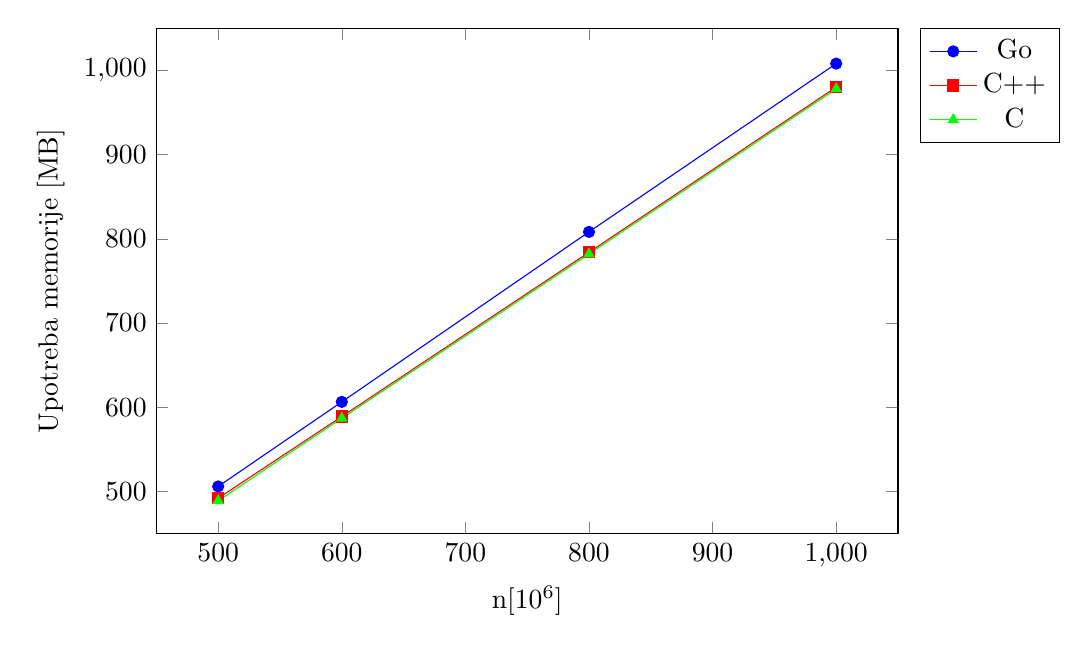
\begin{tikzpicture}
\begin{axis}[
    xlabel={n[$10^{6}$]},
    ylabel={Upotreba memorije [MB]},
    xmin=450, xmax=1050,
    ymin=450, ymax=1050,
    xtick={500,600,700,800,900,1000},
    ytick={500,600,700,800,900,1000},
    legend pos=outer north east,
    ymajorgrids=true,
    grid=none,
    width=11cm,
    height=8cm,
]
\addplot[blue,mark=*] coordinates {(500,506 )(600,606.4)(800,808.2)(1000,1008 )}; 
\addplot[red,mark=square* ]coordinates {(500,492)(600,589)(800,784)(1000,980 )}; 
\addplot[green,mark=triangle*] coordinates {(500,489 )(600,587)(800,782 )(1000, 978)}; 
\legend{Go, C++,C}
\end{axis}
\end{tikzpicture}

\caption{Grafik maksimalne upotrebe memorije različitih implementacija Eratostenovog sita za različito n}
\label{fig:prime2}
\end{center}
\end{figure}


Dužine implementacija su prikazane u tabeli \ref{tab:prime2}. I u ovom primeru najkraća implementacija je u Python-u dok je u C-u najduža. Go se ponovo nalazi između C-a i C++-a po broju linija k\^{o}da.

\begin{table}
\begin{center}
\caption{Dužine k\^{o}da implementacija Eratostenovog sita}
\begin{tabular}{|c|c|c|c|c|}
\hline
		&  C  		&Go 	& C++ & Python 	 \\ \hline
Br. linija koda& 89		& 78	&61	&42		 \\ \hline
\end{tabular}
\label{tab:prime2}
\end{center}
\end{table}

\subsection{Zaključak}

Za ovaj algoritam Go implementacija se ispostavila kao vremenski najefikasnija sa značajnim ubrzanjem u odnosu na sekvencijalno izvršavanje. Upotreba memorije je približno ista kolika je i kod C-a i C++-a kao i dužina k\^{o}da implementacije.


\section{Složeniji primer u programskom jeziku Go}




\chapter{Zaključak}





\printbibliography 
% ==============================================================================
% Završni deo teze i prilozi
\backmatter
% ==============================================================================



\end{document}
